\documentclass[slidestop,compress,mathserif,9pt]{beamer}
\usetheme{CambridgeUS}
\usecolortheme{orchid}
\usepackage{url}
\usepackage{multimedia}
\usepackage{graphicx}
\usepackage{amsfonts,amssymb}
\usepackage{epsfig}
\usepackage{latexsym}
\usepackage[all]{xy}
\usepackage{amsmath}
\usepackage{amsfonts}
\usepackage{amssymb}
\def\mc{\mathcal}
\def\A{\mc{A}}
\def\R{\mathbb R}
\def\K{\mc{K}}
\def\V{\mathbb V}
\def\L{\mathbb L}
\def\Q{\mc{Q}}
\def\N{\mathbb N}
\def\Z{\mc{Z}}
\def\B{\mathbb B}
\def\S{\mathbb S}
\def\C{\mathbb C}
\def\D{\mc{D}}
\def\E{\mc{E}}
%\def\Q{\mathbb Q}
%\def\D{\mathbb D}
%\def\K{\mathbb K}
\def\O{\mathcal{O}}
\def\H{\mathbb H}
\def\M{\mathcal{M}}
\def\m{\mathbb{M}}
%\def\M{\mathbb M}
\def\R{\mc{R}}
\def\T{\mathcal T}
\def\G{\mathcal G}
\def\I{\mc{I}}
\def\F{\mathcal F}
\def\S{\mathcal{S}}
\def\U{\mc{U}}
\def\f{\frac}
\def\lb{\lambda}
\def\r{\rho}
\def\g{\Gamma}
\def\al{\alpha}
\def\lbr{\lbrace}
\def\rbr{\rbrace}
\def\th{\theta}
\def\b{\begin{center}}
\def\e{\end{center}}
\def\be{\begin{enumerate}}
\def\ee{\end{enumerate}}
\parskip 0.2cm
\setbeamercolor{title}{fg=green!45!black}
\setbeamercolor{frametitle}{fg=green!45!black}
\setbeamercolor{itemize item}{fg=white!40!black}
\setbeamercolor{block title}{fg=white!50!black}
\usepackage{setspace}
\setstretch{1.3}
\begin{document}
\title{A Simple Trading Strategy: Implemented using Python}
\author{Gouri Shankar Seal}
\institute{PhD Candidate (May, 2017), Department of Mathematics, Northeastern University, Boston, MA, USA}

\begin{frame}
\titlepage
\end{frame}



\begin{frame}
\frametitle{Organization of Presentation}
\be
\item
Moving averages.
\item
RSI.
\item
Bollinger Bands.
\item
Swing low's and high's.
\item 
The Strategy.
\item
Algorithm for Implementation of the Strategy.
\item 
Backtesting on Historical Data.
\item
Returns and Sharpe Ratio.
\item
Conclusions and Future works.

\ee

\end{frame}

\begin{frame}
\frametitle{Moving Averages}


\be

\item

A $q$-\textbf{day moving average} for a time series $\lbrace x_t \rbrace$ is the average over the past $q$ days
\begin{eqnarray*}
MA^q = \frac{1}{q} \sum_{i=0}^{q-1} x_{t-i}
\end{eqnarray*}

\item
Moving averages smooth a series and helps identify trends. 
\item
\textbf{Short-term or Faster:} $MA^q$ for smaller $q$, captures local trends.
\item
\textbf{Long-term or Slower:} $MA^q$ for larger $q$, captures long-term trends.
\item
\textbf{Crossover Trends:} For $q_1 < q_2$ 
\be
\item $MA^{q_1} > MA^{q_2}$. Market \textbf{Bullish}. Enter Long position. 
\item $MA^{q_1} < MA^{q_2}$. Market \textbf{Bearish}. Go Short.
\ee

\item
Popular short-time moving averages: $MA^{15}, MA^{20}, MA^{50}$. Popular long-time moving averages: $MA^{150}, MA^{200}$.
\ee

\end{frame}

\begin{frame}
\frametitle{Relative Strength Index: RSI}

\be
\item
RSI indicates \emph{upcoming reversal of trends}.

\item
Let RS = Average of $n$ days up-closes/{Average of $n$ days down-closes}. Then
\begin{eqnarray*}
RSI= 100 - \frac{100}{1+RS}.
\end{eqnarray*}
Usually, $n=14$.

\item
$\mathbf{RSI \ge 70}$: Security overbought(or undersold); go Short. 
\item 
$\mathbf{RSI \le 30}$: Security underbought(or oversold); go Long. 

\item
RSI works best when compared with a shorter time moving averages $MA^q$.


\ee


\end{frame}





\begin{frame}

\frametitle{Bollinger Bands}

\be

\item
Let $S_t$ denote the series of closing prices of a security $S$ and $MA^q$ denote the $q$-period moving average of $S_t$.
\item
For any $q$ and $k$:
\begin{eqnarray*}
\underbrace{MA^q - k\sigma}_\text{Lower Bollinger Band} \le MA^q \le \underbrace{MA^q + k\sigma}_\text{Upper Bolliger Band}
\end{eqnarray*}
where, $\sigma = stdev(S_t)$ is the standard deviation. Popular choices are $q=20$, $k=2$.
\item
\textbf{Bandwidth:} $2k\sigma$: indicates the volatility of the security. For more volatile securities greater bandwidth.
\item
\textbf{Signals:} Trend reversal occurs when prices touch the Bollinger Bands.
\be
\item \textbf{Buy Signal}: $S_t \le MA^q - k\sigma$.
\item \textbf{Sell Signal}: $S_t \ge MA^q - k\sigma$.
\ee
\item
Like RSI, Buy/Sell signals are better captured using Bollinger Bands, when used together with moving average crossovers.



\ee


\end{frame}


\begin{frame}

\frametitle{Swing low's and high's}

\be


\item
For a time series of an asset $S_t$ denote 
\be
\item $S_t^{L}$: Series for the daily lows.
\item $S_t^H$: Series for the daily highs
\ee


\item

\textbf{Swing Low:} $S_t^{L}$ is a swing low if its a local minima i.e., 
\begin{eqnarray*}
S_t^{L} \le S_{t-1}^{L} \ \& \ S_t^{L} \le S_{t+1}^{L}.
\end{eqnarray*}

\item

\textbf{Swing High:} $S_t^{H}$ is a swing high if its a local maxima i.e., 
\begin{eqnarray*}
S_t^{H} \ge S_{t-1}^{H} \ \& \ S_t^{H} \ge S_{t+1}^{H}.
\end{eqnarray*}
\item
\textbf{Uptrend Signal:} Higher swing high's and higher swing low's.
\item
\textbf{Stop-loss order:} Usually issued on Long position, set just below the most recent swing low.
\item
During an uptrend: $S_{t_1}^{L} \le S_{t_2}^{L} \le \ldots \le S_{t_k}^L$ for $t_1 < t_2 < \ldots < t_k$, place Stop orders below each $S_{t_i}^L$.

\ee
\end{frame}


\begin{frame}

\frametitle{The Strategy}

\vspace{0.5in}

\b
\emph{When a price is within $2\%$ of a prior swing low and exceeds the lower Bollinger Band with an RSI of atmost 30 and the $20$-day moving average is atleast $5\%$ above the current price enter Long at the current price. Exit at the current price if price falls more than $1\%$ below the swing low.}
\e



\end{frame}






\begin{frame}

\frametitle{The Strategy: Mathematical details}

\be

\item
Let at current time $t$ price be $S_t$ 
\item For some $t^{\prime} \le t$ let the prior swing low be $S_{t^{\prime}}^L$ 
\item The lower Bollinger Band at $t$ be $BB_L(t)$
\item $20$-day moving average at $t$ be $N(t)$
\item $RSI$ for $n=14$ at time $t$ be $RSI(t)$

Then enter Long position at $S_t$ if the following conditions are met:
\begin{eqnarray}
S_t &\le& 1.02S_{t^{\prime}}^L\quad \& \quad S_t \ge BB_L(t)\\
RSI(t) &\le& 30 \quad \& \quad N(t) \ge 1.05 S_t
\end{eqnarray}
 
Exit Long position at current price if price falls $1\%$ below swing low i.e.,
\begin{center}
$S_t \le 0.99S_{t^{\prime}}^L$
\end{center}


\ee







\end{frame}




\begin{frame}[allowframebreaks]

\frametitle{Algorithm for Implementing the Strategy:}

\be
\item
Get Historical data over time frame $[0,T]$ and find all the swing lows:
\begin{center} $S_{t_1}^L \le S_{t_2}^L \le \ldots \le S_{t_k}^L$  \end{center}
\item
\textbf{Iteration over $t_i$:} For any $t_i \in \lbrace t_1,\ldots,t_k \rbrace$ consider the swing low $S_{t_i}^L$ and the price data $S_t$ for $t \in [t_i,t_{i+1})$ and find the set of prices (depending on $[t_i,t_{i+1}]$)
\begin{center}
$Q = \lbrace S_{t_{i_1}},S_{t_{i_2}},\ldots,S_{t_{i_j}}  \rbrace$
\end{center} 
satisfying conditions given by equation $(1)$ and $(2)$
\item
If $Q$ is a non empty set enter Long on Date $t=t_{i_s}$ at the price
\begin{center}
$S_{t_{i_s}} = min(Q)$
\end{center}
for some $t_{i_1} \le s \le t_{i_j}$
\item
Set Sell-Stop order(Stop order) at  $ 1\% $ below the swing low $S_{t_i}^L$ i.e., set
\b $\mbox{Stop order} = 0.99 S_{t_i}^L$\e



\framebreak

\item

\textbf{Case 1:} If a new swing low is achieved that is greater than prior swing low \b$S_{t_{i+1}}^L > S_{t_{i}}^L$ \e
Increase Sell-Stop Order to $1\%$ below $S_{t_{i+1}}^L$ i.e., set
\b $\mbox{Stop order} = 0.99 S_{t_{i+1}}^L$  \e
\item
\textbf{Case 2:} If a new swing low is achieved that is lower than the prior swing low, i.e., \b $S_{t_{i+1}}^L < S_{t_i}^L$   \e
\be
\item
If current price falls $1\%$ below current $\mbox{Stop order}$ then exit Long position at Stop order.
\ee
\item
Check whether current price $S_t$ satisfies the conditions of Equation $(1)$ and $(2)$
\item
If Yes, Enter new Long position at current price $S_t$, and set new Sell-Stop order at $1\%$ below the new swing low $S_{t_{i+1}}^L$.

\ee

\end{frame}


\begin{frame}

\frametitle{Backtesting on Historical market data}
\be
\item
\textbf{Data:} \emph{'INTC','MSFT','AMZN'} stocks, Closing prices.
\item
\textbf{Time frame:} start = '2014-01-01' ; end = '2016-09-30'
\item
\textbf{Moving Average $N(t) = MA^q(t)$:} Taken for $q=20$-days
\item
\textbf{RSI:} Calculated for $n=14$ days window.
\item
\textbf{Bollinger Bands:} $MA^q \pm k\sigma$ with $k=2$. (Actually used $k=0.5$)


\ee

\end{frame}


\begin{frame}

\frametitle{A Time Series Plot: 'INTC', '2014-01-01'-'2016-09-30'}

\begin{figure}
\includegraphics[scale=0.2]{intc.png}
\caption{TIme Series Plot: Ticker: 'INTC' with 'RSI'}
\end{figure}





\end{frame}



\begin{frame}[allowframebreaks]

\frametitle{Trading Signals on INTC Stocks from 2014-01-01 to 2016-09-30:}
\small{
Enter first long position on 2014-02-04 at \$ 23.82\\
Sell-stop order now at \$ 24.4332\\
\hrulefill \\
Exit Long position on 2014-02-03 at \$ 23.950001\\
\hrulefill \\
Enter new long on 2014-02-05 at \$ 23.52\\
Sell-stop order decreased on 2014-02-05 to \$ 23.2848\\
\hrulefill\\
Sell-stop order increased on 2014-02-19 to \$ 24.255\\
\hrulefill\\
Sell-stop order increased on 2014-02-25 to \$ 24.37380099\\
\hrulefill\\
Sell-stop order increased on 2014-02-27 to \$ 24.5124\\
$\ldots  \quad \ldots \quad  \ldots \ldots  \quad \ldots \quad  \ldots \ldots  \quad \ldots \quad  \ldots \ldots  \quad \ldots \quad  \ldots  \ldots  \quad \ldots \quad  \ldots \ldots  \quad \ldots \quad  \ldots \ldots  $ \\
Exit Long position on 2015-10-29 at \$ 34.029999\\
\hrulefill\\
Enter new long on 2015-11-13 at \$ 32.110001\\
Sell-stop order decreased on 2015-11-13 to \$ 33.52140099\\
\hrulefill\\
Exit Long position on 2015-11-09 at \$ 33.349998\\
\hrulefill\\
Enter new long on 2015-11-16 at \$ 32.099998\\
Sell-stop order decreased on 2015-11-16 to \$ 31.77899802\\
\hrulefill\\

Sell-stop order increased on 2015-11-24 to \$ 34.01640099\\
\hrulefill\\
Sell-stop order increased on 2015-12-08 to \$ 34.4025\\
$\ldots  \quad \ldots \quad  \ldots \ldots  \quad \ldots \quad  \ldots \ldots  \quad \ldots \quad  \ldots \ldots  \quad \ldots \quad  \ldots  \ldots  \quad \ldots \quad  \ldots \ldots  \quad \ldots \quad  \ldots \ldots  $ \\
Sell-stop order increased on 2016-09-13 to \$ 35.25390099\\
\hrulefill\\
Sell-stop order increased on 2016-09-20 to \$ 36.76859901\\
\b
\textbf{Close out position:} Go Short on Stop-order at \$ 36.76859901  
\e
}




\end{frame}


\begin{frame}[allowframebreaks]

\frametitle{Performance Metrics: Strategy return and Market return: Sharpe Ratio}

\be
\item
$\mbox{Vector of Simple Strategy Returns} = [(M_{t+1} - M_{t})/{M_{t}}]_{t=1}^n$, where $M_{t+1}$ is Short position at $t+1$ preceded by Long position $M_t$ at $t$.
\item
Define \emph{time-weighted} $\mbox{True Strategy Return} = r$ as: \b$ 1+r = \prod_{t=1}^n \frac{M_{t+1} -M_t}{M_t} = (M_2-M_1)/{M_1} \times \ldots \times (M_{n+1} - M_n)/{M_n}$\e
\item
\textbf{Sharpe Ratio:}(Measure of reward to risk) $\quad S = \frac{\sqrt{n}Avg(d)}{Std(d)}$, where, $d = $ vector of daily market return for a period of $n$ days and Avg and Std are Average and Standard deviation of $d$.

\item Tabulated below is a Comparison between the True Strategy return ($r$) and the Sharpe ratio ($S$) calculated from Market return data between '2014-01-01' and '2016-09-30', $n=693:$ \\  
\begin{center}
\begin{tabular}{ l | c | r }
\hline
  Stocks & True Strategy Return(r) & Sharpe Ratio \\ \hline
  'INTC' & 0.99 & 1.17 \\ \hline
  'MSFT' & 1.00 & 1.30 \\ \hline
  'AMZN' & 1.00  & 1.64
\end{tabular}
\end{center}

\framebreak


%\end{frame}


%\begin{frame}

%\frametitle{Plot of Average Periodic Returns from Strategy: 'INTC','MSFT','AMZN'}

\item Plot the vector of the average periodic returns obtained from the Signals.

\begin{figure}
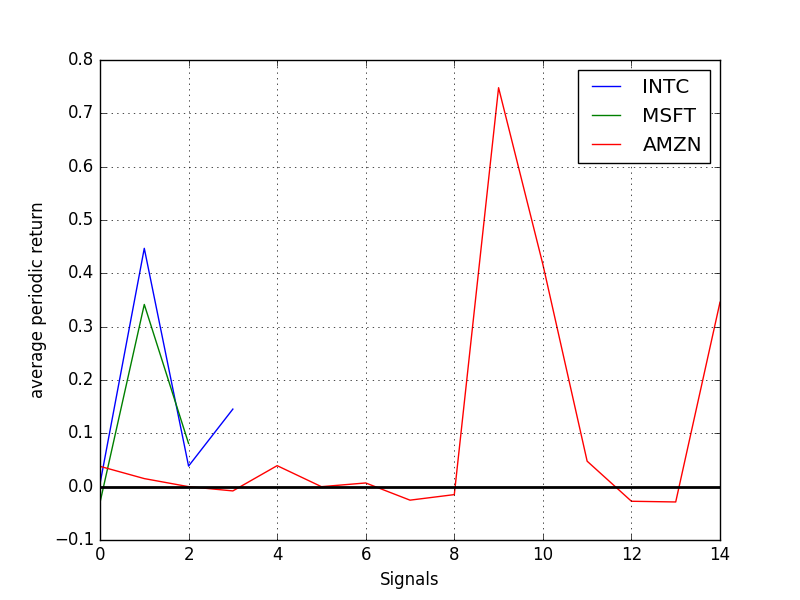
\includegraphics[scale=0.3]{returns.png}
\caption{Average Periodic Returns}
\end{figure}

\ee


\end{frame}


\begin{frame}
\frametitle{Conclusion and Future works:}

\small{

\textbf{Strategy Advantages:}
\be
\item
\textbf{Implementation:} Easy to implement.
\item
\textbf{Robust:} Takes account of not only moving average crossover trend but also important index like RSI
and Bollinger bands.
\item
\textbf{Monitoring:} Can be easily automated and does not require constant monitoring like in day trading.
\ee
\textbf{Strategy Disadvantages:}
\be
\item
\textbf{Trading Signals:} Trading Signals are fewer in number, can lead to significant loss.
\textbf{Operation time:} Longer operation time than simpler strategies.
\ee
\textbf{Further Performance Statistics:}
\be
\item 
\textbf{Risk Analysis:}
Perform risk analysis, robust risk-adjusted returns (Drawdown) 
\item
\textbf{Optimization:} Calibrate parameter set $\mathcal{P}= $(RSI window, Bandwidth, distance from swing low, MA crossover) to maximize returns. Monte Carlo simulations to select starting points.
\ee

}













\end{frame}


































































































































































































































































































































































 




































































\end{document}
